% $Author: oscar $
% $Date: 2009-09-15 16:53:48 +0200 (Tue, 15 Sep 2009) $
% $Revision: 29111 $
%=================================================================
\ifx\wholebook\relax\else
% --------------------------------------------
% Lulu:
	\documentclass[a4paper,10pt,twoside]{book}
	\usepackage[
		papersize={6.13in,9.21in},
		hmargin={.815in,.815in},
		vmargin={.98in,.98in},
		ignoreheadfoot
	]{geometry}
	\usepackage[hangul]{kotex}
	% $Author: oscar $
% $Date: 2009-09-13 20:58:29 +0200 (Sun, 13 Sep 2009) $
% $Revision: 29070 $
%=============================================================
% NB: documentclass must be set in main document.
% Allows book to be generated in multiple formats.
%=============================================================
%:Packages
\usepackage[T1]{fontenc}  %%%%%really important to get the code directly in the text!
\usepackage{palatino}
\usepackage{ifthen}
\usepackage{graphicx}
\graphicspath{{figures/}}
\usepackage{xspace}
\usepackage{makeidx}
\usepackage{isodateo} % enable \isodate
\usepackage{amssymb,textcomp}
%=============================================================
%:More packages
%\usepackage[english]{babel}
%\usepackage{lmodern}
%\usepackage[scaled=0.85]{helvet}
%\usepackage{microtype}
%\usepackage{theorem}
%\usepackage{float}
%\usepackage{longtable}
%\usepackage[nottoc]{tocbibind}
%\usepackage{multicol}
%\usepackage{booktabs}	% book-style tables
%\usepackage{topcapt}	% enables \topcaption
%\usepackage{multirow}
%\usepackage{tabularx}
%\usepackage{alltt}
\usepackage[usenames,dvipsnames]{color}
%\usepackage[hang]{subfigure}\makeatletter\def\p@subfigure{\thefigure\,}\makeatother
%\usepackage{rotating}
%\usepackage{enumitem}	% apb: allows more control over tags in enumerations
%\usepackage{verbatim}     % for comment environment
%\usepackage{varioref}	% for page references that work
%\usepackage{needspace}
%\usepackage[newparttoc]{titlesec}
%\usepackage{titletoc}
%\usepackage{wrapfig}
\usepackage[
	colorlinks=true,
	linkcolor=black,
	urlcolor=black,
	citecolor=black
]{hyperref}   % should come last
%=============================================================
%:URL style
\makeatletter
\def\url@leostyle{%
  \@ifundefined{selectfont}{\def\UrlFont{\sf}}{\def\UrlFont{\sffamily}}}
\makeatother
\urlstyle{leo}
%=============================================================
%:Booleans
\newboolean{lulu}
\setboolean{lulu}{false}
\newcommand{\ifluluelse}[2]{\ifthenelse{\boolean{lulu}}{#1}{#2}}
%=============================================================
%:Editorial comment macros
\newcommand{\nnbb}[2]{
  \fbox{\bfseries\sffamily\scriptsize#1}
  {\sf\small$\blacktriangleright$\textit{#2}$\blacktriangleleft$}
}
\newcommand{\on}[1]{\nnbb{Oscar}{#1}}
\newcommand{\here}{\nnbb{CONTINUE}{HERE}}
%=============================================================
%:Abbreviation macros
\newcommand{\ie}{\emph{i.e.},\xspace}
\newcommand{\eg}{\emph{e.g.},\xspace}
\newcommand{\etc}{\emph{etc.}\xspace}
\newcommand{\etal}{\emph{et al.}\xspace}
\newcommand{\straightquote}{"}
\newcommand{\sba}{\url{SquareBracketAssociates.org}\xspace}
%=============================================================
%:Patterns
% \newcommand{\pattern}[2]{\newpage\section{{\sf #1}}\label{pat:#2}}
% \newcommand{\pattern}[2]{\newpage\index{#1 (Pattern)}\section{#1}\label{pat:#2}}
\newcommand{\pattern}[2]{\cleardoublepage\index{#1 (패턴)}\section{#1}\label{pat:#2}}
\newcommand{\thumbnail}[2]{\index{#1 (패턴)}\subsection{#1}\label{pat:#2}}
\newcommand{\thumblang}[2]{\index{#1 (패턴 랭귀지)}\subsection{#1}\label{pat:#2}}
\newcommand{\variant}[1]{{\emph{#1}}\xspace}
% \newcommand{\problem}[1]{\subsection*{Problem}\emph{#1}}
\newcommand{\intent}[1]{\paragraph{의도}\emph{#1}}
\newcommand{\problem}[1]{\paragraph{문제}\emph{#1}}
\newcommand{\solution}[1]{\paragraph{해결}\emph{#1}}
\newcommand{\discussion}[0]{\paragraph{토론}}
\newcommand{\cmd}[1]{{\tt #1}\xspace}
%=============================================================
%:Environments
\newenvironment{bulletlist}{\begin{itemize}\setlength{\itemsep}{0ex}}
{\end{itemize}}
%=============================================================
%:Cross reference macros
\newcommand{\chalabel}[1]{\label{cha:#1}}
\newcommand{\seclabel}[1]{\label{sec:#1}}
\newcommand{\figlabel}[1]{\label{fig:#1}}
\newcommand{\tablabel}[1]{\label{tab:#1}}
\newcommand{\rulelabel}[1]{\label{rule:#1}}
\newcommand{\eglabel}[1]{\label{eg:#1}}
\newcommand{\scrlabel}[1]{\label{scr:#1}}
\newcommand{\mthlabel}[1]{\label{mth:#1}}
\newcommand{\clslabel}[1]{\label{cls:#1}}
\newcommand{\faqlabel}[1]{\label{faq:#1}}
%\newcommand{\charef}[1]{Chapter~\ref{cha:#1}\xspace}
%\newcommand{\secref}[1]{Section~\ref{sec:#1}\xspace}
\newcommand{\figref}[1]{Figure~\ref{fig:#1}\xspace}
% \newcommand{\patpgref}[2]{\hyperref[pat:#2]{\sf #1} [p.~\pageref{pat:#2}]\xspace}
\newcommand{\patpgref}[2]{\index{#1 (Pattern)}\hyperref[pat:#2]{#1} [p.~\pageref{pat:#2}]\xspace}
\newcommand{\patlangpgref}[2]{\index{#1 (Pattern language)}\hyperref[pat:#2]{#1} [p.~\pageref{pat:#2}]\xspace}
% \newcommand{\patref}[2]{\hyperref[pat:#2]{\sf #1}\xspace}
\newcommand{\patref}[2]{\index{#1 (Pattern)}\hyperref[pat:#2]{#1}\xspace}
\newcommand{\patlangref}[2]{\index{#1 (Pattern language)}\hyperref[pat:#2]{#1}\xspace}
% \newcommand{\charef}[2]{\hyperref[cha:#2]{\underline{\sf #1}}\xspace}
% \newcommand{\charef}[2]{\hyperref[cha:#2]{\sf #1}\xspace}
\newcommand{\charef}[2]{\index{#1 (Pattern cluster)}\hyperref[cha:#2]{#1}\xspace}
% \newcommand{\chapgref}[2]{\hyperref[cha:#2]{\sf #1} [p.~\pageref{cha:#2}]\xspace}
\newcommand{\chapgref}[2]{\index{#1 (Pattern cluster)}\hyperref[cha:#2]{#1} [p.~\pageref{cha:#2}]\xspace}
%\newcommand{\Figref}[1]{Figure~\ref{fig:#1}\xspace}
%\newcommand{\appref}[1]{Appendix~\ref{app:#1}\xspace}
%\newcommand{\tabref}[1]{Table~\ref{tab:#1}\xspace}
%\newcommand{\ruleref}[1]{\ref{rule:#1}\xspace}
%\newcommand{\egref}[1]{example~\ref{eg:#1}\xspace}
%\newcommand{\Egref}[1]{Example~\ref{eg:#1}\xspace}
%\newcommand{\scrref}[1]{script~\ref{scr:#1}\xspace}
%\newcommand{\Scrref}[1]{Script~\ref{scr:#1}\xspace}
%\newcommand{\tscrref}[1]{the script~\ref{scr:#1}\xspace}
%\newcommand{\Tscrref}[1]{The script~\ref{scr:#1}\xspace}
%\newcommand{\mthref}[1]{method~\ref{mth:#1}\xspace}
%\newcommand{\mthsref}[1]{methods~\ref{mth:#1}\xspace}
%\newcommand{\Mthref}[1]{Method~\ref{mth:#1}\xspace}
%\newcommand{\tmthref}[1]{the method~\ref{mth:#1}\xspace}
%\newcommand{\Tmthref}[1]{The method~\ref{mth:#1}\xspace}
%\newcommand{\clsref}[1]{class~\ref{cls:#1}\xspace}
%\newcommand{\tclsref}[1]{the class~\ref{cls:#1}\xspace}
%\newcommand{\Tclsref}[1]{The class~\ref{cls:#1}\xspace}
%=============================================================
%:Page Layout
\setlength{\headsep}{1cm}
%=============================================================
%:Menu item macro
%\definecolor{lightgray}{gray}{0.89}
%\newcommand{\menu}[1]{{%
%	\setlength{\fboxsep}{0pt}%
%	\colorbox{lightgray}{{{\upshape\sffamily\strut \,#1\,}}}}}
%\newcommand{\go}{\,$\triangleright$\,}
%\newcommand{\short}[1]{\mbox{{\sc cmd}\hspace{0.08em}--\hspace{0.09em}#1}\xspace}
%\newcommand{\button}[1]{{%
%	\setlength{\fboxsep}{0pt}%
%	\fbox{{\upshape\sffamily\strut \,#1\,}}}}
%\newcommand{\toolsflap}{\textit{Tools} flap\xspace}
%=============================================================
%:Section depth
%\setcounter{secnumdepth}{2}
%
%\DeclareGraphicsExtensions{.pdf, .jpg, .png}
%=============================================================
%:PDF setup
\hypersetup{
   pdftitle={Object-Oriented Reengineering Patterns},
   pdfauthor={Serge Demeyer, St\'ephane Ducasse, Oscar Nierstrasz},
   pdfkeywords={Reengineering, Object-Oriented Programming, Patterns},
   pdfsubject={Computer Science}
}
%=============================================================
%:Page layout and appearance
%\renewcommand{\chaptermark}[1]{\markboth{#1}{}}
%\renewcommand{\sectionmark}[1]{\markright{\thesection\ #1}}
%\renewpagestyle{plain}[\small\itshape]{%
%	\setheadrule{0pt}%
%	\sethead[][][]{}{}{}%
%	\setfoot[][][]{}{}{}}
%\renewpagestyle{headings}[\small\itshape]{%
%	\setheadrule{0pt}%
%	\setmarks{chapter}{section}%
%	\sethead[\thepage][][\chaptertitle]{\sectiontitle}{}{\thepage}%
%	\setfoot[][][]{}{}{}}
%=============================================================
%:Title section setup and TOC numbering depth
%\setcounter{secnumdepth}{1}
%\setcounter{tocdepth}{1}
%\titleformat{\part}[display]{\centering}{\huge\partname\ \thepart}{1em}{\Huge\textbf}[]
%\titleformat{\chapter}[display]{}{\huge\chaptertitlename\ \thechapter}{1em}{\Huge\raggedright\textbf}[]
%\titlecontents{part}[3pc]{%
%		\pagebreak[2]\addvspace{1em plus.4em minus.2em}%
%		\leavevmode\large\bfseries}
%	{\contentslabel{3pc}}{\hspace*{-3pc}}
%	{}[\nopagebreak]
%\titlecontents{chapter}[3pc]{%
%		\pagebreak[0]\addvspace{1em plus.2em minus.2em}%
%		\leavevmode\bfseries}
%	{\contentslabel{3pc}}{}
%	{\hfill\contentspage}[\nopagebreak]
%\dottedcontents{section}[3pc]{}{3pc}{1pc}
%\dottedcontents{subsection}[3pc]{}{0pc}{1pc}
%\let\origdoublepage\cleardoublepage
%\newcommand{\clearemptydoublepage}{%
%  \clearpage
%  {\pagestyle{empty}\origdoublepage}}
%\let\cleardoublepage\clearemptydoublepage % see http://www.tex.ac.uk/cgi-bin/texfaq2html?label=patch
%=============================================================
%:Listings package configuration
\newcommand{\caret}{\makebox{\raisebox{0.4ex}{\footnotesize{$\wedge$}}}}
% \newcommand{\escape}{{\sf \textbackslash}}
\definecolor{source}{gray}{0.95}
\usepackage{listings}
\lstdefinelanguage{Smalltalk}{
  morestring=[d]',
% Adapt this to other languages!
%  morecomment=[s]{"}{"},
  alsoletter={\#:},
  %escapechar={!},
  literate=
    {BANG}{!}1
%    {UNDERSCORE}{\_}1
    {\\st}{Smalltalk}9 % convenience -- in case \st occurs in code
    % {'}{{\textquotesingle}}1 % replaced by upquote=true in \lstset
%    {_}{{$\leftarrow$}}1
    {>>>}{{\sep}}1
    {^}{{$\uparrow$}}1
    {~}{{$\sim$}}1
    {-}{{\sf -\hspace{-0.13em}-}}1  % the goal is to make - the same width as +
    {+}{\raisebox{0.08ex}{+}}1		% and to raise + off the baseline to match -
    {-->}{{\quad$\longrightarrow$\quad}}3
	, % Don't forget the comma at the end!
  tabsize=4
}[keywords,comments,strings]

\lstset{language=Smalltalk,
	basicstyle=\sffamily,
	keywordstyle=\color{black}\bfseries,
	% stringstyle=\ttfamily, % Ugly! do we really want this? -- on
	mathescape=true,
	showstringspaces=false,
	keepspaces=true,
	breaklines=true,
	breakautoindent=true,
	backgroundcolor=\color{source},
	lineskip={-1pt}, % Ugly hack
	upquote=true, % straight quote; requires textcomp package
	columns=fullflexible} % no fixed width fonts
% \newcommand{\ct}{\lstinline[mathescape=false,basicstyle={\sffamily\upshape}]}
\newcommand{\ct}{\lstinline[mathescape=false,backgroundcolor=\color{white},basicstyle={\sffamily\upshape}]}
\newcommand{\lct}[1]{{\textsf{\textup{#1}}}}
%\newcommand{\scat}[1]{\emph{\textsf{#1}}\xspace}
%\newcommand{\prot}[1]{\emph{\textsf{#1}}\xspace}
% NB: No argument!
\lstnewenvironment{code}[0]{%
	\lstset{%
		% frame=lines,
		frame=single,
		framerule=0pt,
		mathescape=false
	}
}{}
%\def\ignoredollar#1{}
%=============================================================
%:Reserving space
%\newcommand{\needlines}[1]{\Needspace{#1\baselineskip}}
%=============================================================
%:Indexing macros
% Macros ending with "ind" generate text as well as an index entry
% Macros ending with "index" *only* generate an index entry
\newcommand{\ind}[1]{\index{#1}#1\xspace} % plain text
\newcommand{\subind}[2]{\index{#1!#2}#2\xspace} % show #2, subindex under #1
\newcommand{\emphind}[1]{\index{#1}\emph{#1}\xspace} % emph #1
\newcommand{\emphsubind}[2]{\index{#1!#2}\emph{#2}\xspace} % show emph #2, subindex under #1
\newcommand{\patind}[1]{\index{#1@#1 (pattern)}\ct{#1}\xspace} % pattern
\newcommand{\seeindex}[2]{\index{#1|see{#2}}} % #1, see #2
%\newcommand{\boldidx}[1]{{\bf #1}} % breaks hyperlink
%\newcommand{\indmain}[1]{\index{#1}#1\xspace} 
%\newcommand{\emphsubindmain}[2]{\index{#1!#2}\emph{#2}\xspace} % subindex, main entry
%\newcommand{\subindmain}[2]{\index{#1!#2}#2\xspace} % subindex, main entry
%\newcommand{\clsindmain}[1]{\index{#1!\#@(class)}\ct{#1}\xspace} % class main
%\newcommand{\indexmain}[1]{\index{#1}} 
%=============================================================
\parskip 1ex
%=============================================================

	\pagestyle{headings}
	\setboolean{lulu}{true}
% --------------------------------------------
% A4:
%	\documentclass[a4paper,11pt,twoside]{book}
%	% $Author: oscar $
% $Date: 2009-09-13 20:58:29 +0200 (Sun, 13 Sep 2009) $
% $Revision: 29070 $
%=============================================================
% NB: documentclass must be set in main document.
% Allows book to be generated in multiple formats.
%=============================================================
%:Packages
\usepackage[T1]{fontenc}  %%%%%really important to get the code directly in the text!
\usepackage{palatino}
\usepackage{ifthen}
\usepackage{graphicx}
\graphicspath{{figures/}}
\usepackage{xspace}
\usepackage{makeidx}
\usepackage{isodateo} % enable \isodate
\usepackage{amssymb,textcomp}
%=============================================================
%:More packages
%\usepackage[english]{babel}
%\usepackage{lmodern}
%\usepackage[scaled=0.85]{helvet}
%\usepackage{microtype}
%\usepackage{theorem}
%\usepackage{float}
%\usepackage{longtable}
%\usepackage[nottoc]{tocbibind}
%\usepackage{multicol}
%\usepackage{booktabs}	% book-style tables
%\usepackage{topcapt}	% enables \topcaption
%\usepackage{multirow}
%\usepackage{tabularx}
%\usepackage{alltt}
\usepackage[usenames,dvipsnames]{color}
%\usepackage[hang]{subfigure}\makeatletter\def\p@subfigure{\thefigure\,}\makeatother
%\usepackage{rotating}
%\usepackage{enumitem}	% apb: allows more control over tags in enumerations
%\usepackage{verbatim}     % for comment environment
%\usepackage{varioref}	% for page references that work
%\usepackage{needspace}
%\usepackage[newparttoc]{titlesec}
%\usepackage{titletoc}
%\usepackage{wrapfig}
\usepackage[
	colorlinks=true,
	linkcolor=black,
	urlcolor=black,
	citecolor=black
]{hyperref}   % should come last
%=============================================================
%:URL style
\makeatletter
\def\url@leostyle{%
  \@ifundefined{selectfont}{\def\UrlFont{\sf}}{\def\UrlFont{\sffamily}}}
\makeatother
\urlstyle{leo}
%=============================================================
%:Booleans
\newboolean{lulu}
\setboolean{lulu}{false}
\newcommand{\ifluluelse}[2]{\ifthenelse{\boolean{lulu}}{#1}{#2}}
%=============================================================
%:Editorial comment macros
\newcommand{\nnbb}[2]{
  \fbox{\bfseries\sffamily\scriptsize#1}
  {\sf\small$\blacktriangleright$\textit{#2}$\blacktriangleleft$}
}
\newcommand{\on}[1]{\nnbb{Oscar}{#1}}
\newcommand{\here}{\nnbb{CONTINUE}{HERE}}
%=============================================================
%:Abbreviation macros
\newcommand{\ie}{\emph{i.e.},\xspace}
\newcommand{\eg}{\emph{e.g.},\xspace}
\newcommand{\etc}{\emph{etc.}\xspace}
\newcommand{\etal}{\emph{et al.}\xspace}
\newcommand{\straightquote}{"}
\newcommand{\sba}{\url{SquareBracketAssociates.org}\xspace}
%=============================================================
%:Patterns
% \newcommand{\pattern}[2]{\newpage\section{{\sf #1}}\label{pat:#2}}
% \newcommand{\pattern}[2]{\newpage\index{#1 (Pattern)}\section{#1}\label{pat:#2}}
\newcommand{\pattern}[2]{\cleardoublepage\index{#1 (패턴)}\section{#1}\label{pat:#2}}
\newcommand{\thumbnail}[2]{\index{#1 (패턴)}\subsection{#1}\label{pat:#2}}
\newcommand{\thumblang}[2]{\index{#1 (패턴 랭귀지)}\subsection{#1}\label{pat:#2}}
\newcommand{\variant}[1]{{\emph{#1}}\xspace}
% \newcommand{\problem}[1]{\subsection*{Problem}\emph{#1}}
\newcommand{\intent}[1]{\paragraph{의도}\emph{#1}}
\newcommand{\problem}[1]{\paragraph{문제}\emph{#1}}
\newcommand{\solution}[1]{\paragraph{해결}\emph{#1}}
\newcommand{\discussion}[0]{\paragraph{토론}}
\newcommand{\cmd}[1]{{\tt #1}\xspace}
%=============================================================
%:Environments
\newenvironment{bulletlist}{\begin{itemize}\setlength{\itemsep}{0ex}}
{\end{itemize}}
%=============================================================
%:Cross reference macros
\newcommand{\chalabel}[1]{\label{cha:#1}}
\newcommand{\seclabel}[1]{\label{sec:#1}}
\newcommand{\figlabel}[1]{\label{fig:#1}}
\newcommand{\tablabel}[1]{\label{tab:#1}}
\newcommand{\rulelabel}[1]{\label{rule:#1}}
\newcommand{\eglabel}[1]{\label{eg:#1}}
\newcommand{\scrlabel}[1]{\label{scr:#1}}
\newcommand{\mthlabel}[1]{\label{mth:#1}}
\newcommand{\clslabel}[1]{\label{cls:#1}}
\newcommand{\faqlabel}[1]{\label{faq:#1}}
%\newcommand{\charef}[1]{Chapter~\ref{cha:#1}\xspace}
%\newcommand{\secref}[1]{Section~\ref{sec:#1}\xspace}
\newcommand{\figref}[1]{Figure~\ref{fig:#1}\xspace}
% \newcommand{\patpgref}[2]{\hyperref[pat:#2]{\sf #1} [p.~\pageref{pat:#2}]\xspace}
\newcommand{\patpgref}[2]{\index{#1 (Pattern)}\hyperref[pat:#2]{#1} [p.~\pageref{pat:#2}]\xspace}
\newcommand{\patlangpgref}[2]{\index{#1 (Pattern language)}\hyperref[pat:#2]{#1} [p.~\pageref{pat:#2}]\xspace}
% \newcommand{\patref}[2]{\hyperref[pat:#2]{\sf #1}\xspace}
\newcommand{\patref}[2]{\index{#1 (Pattern)}\hyperref[pat:#2]{#1}\xspace}
\newcommand{\patlangref}[2]{\index{#1 (Pattern language)}\hyperref[pat:#2]{#1}\xspace}
% \newcommand{\charef}[2]{\hyperref[cha:#2]{\underline{\sf #1}}\xspace}
% \newcommand{\charef}[2]{\hyperref[cha:#2]{\sf #1}\xspace}
\newcommand{\charef}[2]{\index{#1 (Pattern cluster)}\hyperref[cha:#2]{#1}\xspace}
% \newcommand{\chapgref}[2]{\hyperref[cha:#2]{\sf #1} [p.~\pageref{cha:#2}]\xspace}
\newcommand{\chapgref}[2]{\index{#1 (Pattern cluster)}\hyperref[cha:#2]{#1} [p.~\pageref{cha:#2}]\xspace}
%\newcommand{\Figref}[1]{Figure~\ref{fig:#1}\xspace}
%\newcommand{\appref}[1]{Appendix~\ref{app:#1}\xspace}
%\newcommand{\tabref}[1]{Table~\ref{tab:#1}\xspace}
%\newcommand{\ruleref}[1]{\ref{rule:#1}\xspace}
%\newcommand{\egref}[1]{example~\ref{eg:#1}\xspace}
%\newcommand{\Egref}[1]{Example~\ref{eg:#1}\xspace}
%\newcommand{\scrref}[1]{script~\ref{scr:#1}\xspace}
%\newcommand{\Scrref}[1]{Script~\ref{scr:#1}\xspace}
%\newcommand{\tscrref}[1]{the script~\ref{scr:#1}\xspace}
%\newcommand{\Tscrref}[1]{The script~\ref{scr:#1}\xspace}
%\newcommand{\mthref}[1]{method~\ref{mth:#1}\xspace}
%\newcommand{\mthsref}[1]{methods~\ref{mth:#1}\xspace}
%\newcommand{\Mthref}[1]{Method~\ref{mth:#1}\xspace}
%\newcommand{\tmthref}[1]{the method~\ref{mth:#1}\xspace}
%\newcommand{\Tmthref}[1]{The method~\ref{mth:#1}\xspace}
%\newcommand{\clsref}[1]{class~\ref{cls:#1}\xspace}
%\newcommand{\tclsref}[1]{the class~\ref{cls:#1}\xspace}
%\newcommand{\Tclsref}[1]{The class~\ref{cls:#1}\xspace}
%=============================================================
%:Page Layout
\setlength{\headsep}{1cm}
%=============================================================
%:Menu item macro
%\definecolor{lightgray}{gray}{0.89}
%\newcommand{\menu}[1]{{%
%	\setlength{\fboxsep}{0pt}%
%	\colorbox{lightgray}{{{\upshape\sffamily\strut \,#1\,}}}}}
%\newcommand{\go}{\,$\triangleright$\,}
%\newcommand{\short}[1]{\mbox{{\sc cmd}\hspace{0.08em}--\hspace{0.09em}#1}\xspace}
%\newcommand{\button}[1]{{%
%	\setlength{\fboxsep}{0pt}%
%	\fbox{{\upshape\sffamily\strut \,#1\,}}}}
%\newcommand{\toolsflap}{\textit{Tools} flap\xspace}
%=============================================================
%:Section depth
%\setcounter{secnumdepth}{2}
%
%\DeclareGraphicsExtensions{.pdf, .jpg, .png}
%=============================================================
%:PDF setup
\hypersetup{
   pdftitle={Object-Oriented Reengineering Patterns},
   pdfauthor={Serge Demeyer, St\'ephane Ducasse, Oscar Nierstrasz},
   pdfkeywords={Reengineering, Object-Oriented Programming, Patterns},
   pdfsubject={Computer Science}
}
%=============================================================
%:Page layout and appearance
%\renewcommand{\chaptermark}[1]{\markboth{#1}{}}
%\renewcommand{\sectionmark}[1]{\markright{\thesection\ #1}}
%\renewpagestyle{plain}[\small\itshape]{%
%	\setheadrule{0pt}%
%	\sethead[][][]{}{}{}%
%	\setfoot[][][]{}{}{}}
%\renewpagestyle{headings}[\small\itshape]{%
%	\setheadrule{0pt}%
%	\setmarks{chapter}{section}%
%	\sethead[\thepage][][\chaptertitle]{\sectiontitle}{}{\thepage}%
%	\setfoot[][][]{}{}{}}
%=============================================================
%:Title section setup and TOC numbering depth
%\setcounter{secnumdepth}{1}
%\setcounter{tocdepth}{1}
%\titleformat{\part}[display]{\centering}{\huge\partname\ \thepart}{1em}{\Huge\textbf}[]
%\titleformat{\chapter}[display]{}{\huge\chaptertitlename\ \thechapter}{1em}{\Huge\raggedright\textbf}[]
%\titlecontents{part}[3pc]{%
%		\pagebreak[2]\addvspace{1em plus.4em minus.2em}%
%		\leavevmode\large\bfseries}
%	{\contentslabel{3pc}}{\hspace*{-3pc}}
%	{}[\nopagebreak]
%\titlecontents{chapter}[3pc]{%
%		\pagebreak[0]\addvspace{1em plus.2em minus.2em}%
%		\leavevmode\bfseries}
%	{\contentslabel{3pc}}{}
%	{\hfill\contentspage}[\nopagebreak]
%\dottedcontents{section}[3pc]{}{3pc}{1pc}
%\dottedcontents{subsection}[3pc]{}{0pc}{1pc}
%\let\origdoublepage\cleardoublepage
%\newcommand{\clearemptydoublepage}{%
%  \clearpage
%  {\pagestyle{empty}\origdoublepage}}
%\let\cleardoublepage\clearemptydoublepage % see http://www.tex.ac.uk/cgi-bin/texfaq2html?label=patch
%=============================================================
%:Listings package configuration
\newcommand{\caret}{\makebox{\raisebox{0.4ex}{\footnotesize{$\wedge$}}}}
% \newcommand{\escape}{{\sf \textbackslash}}
\definecolor{source}{gray}{0.95}
\usepackage{listings}
\lstdefinelanguage{Smalltalk}{
  morestring=[d]',
% Adapt this to other languages!
%  morecomment=[s]{"}{"},
  alsoletter={\#:},
  %escapechar={!},
  literate=
    {BANG}{!}1
%    {UNDERSCORE}{\_}1
    {\\st}{Smalltalk}9 % convenience -- in case \st occurs in code
    % {'}{{\textquotesingle}}1 % replaced by upquote=true in \lstset
%    {_}{{$\leftarrow$}}1
    {>>>}{{\sep}}1
    {^}{{$\uparrow$}}1
    {~}{{$\sim$}}1
    {-}{{\sf -\hspace{-0.13em}-}}1  % the goal is to make - the same width as +
    {+}{\raisebox{0.08ex}{+}}1		% and to raise + off the baseline to match -
    {-->}{{\quad$\longrightarrow$\quad}}3
	, % Don't forget the comma at the end!
  tabsize=4
}[keywords,comments,strings]

\lstset{language=Smalltalk,
	basicstyle=\sffamily,
	keywordstyle=\color{black}\bfseries,
	% stringstyle=\ttfamily, % Ugly! do we really want this? -- on
	mathescape=true,
	showstringspaces=false,
	keepspaces=true,
	breaklines=true,
	breakautoindent=true,
	backgroundcolor=\color{source},
	lineskip={-1pt}, % Ugly hack
	upquote=true, % straight quote; requires textcomp package
	columns=fullflexible} % no fixed width fonts
% \newcommand{\ct}{\lstinline[mathescape=false,basicstyle={\sffamily\upshape}]}
\newcommand{\ct}{\lstinline[mathescape=false,backgroundcolor=\color{white},basicstyle={\sffamily\upshape}]}
\newcommand{\lct}[1]{{\textsf{\textup{#1}}}}
%\newcommand{\scat}[1]{\emph{\textsf{#1}}\xspace}
%\newcommand{\prot}[1]{\emph{\textsf{#1}}\xspace}
% NB: No argument!
\lstnewenvironment{code}[0]{%
	\lstset{%
		% frame=lines,
		frame=single,
		framerule=0pt,
		mathescape=false
	}
}{}
%\def\ignoredollar#1{}
%=============================================================
%:Reserving space
%\newcommand{\needlines}[1]{\Needspace{#1\baselineskip}}
%=============================================================
%:Indexing macros
% Macros ending with "ind" generate text as well as an index entry
% Macros ending with "index" *only* generate an index entry
\newcommand{\ind}[1]{\index{#1}#1\xspace} % plain text
\newcommand{\subind}[2]{\index{#1!#2}#2\xspace} % show #2, subindex under #1
\newcommand{\emphind}[1]{\index{#1}\emph{#1}\xspace} % emph #1
\newcommand{\emphsubind}[2]{\index{#1!#2}\emph{#2}\xspace} % show emph #2, subindex under #1
\newcommand{\patind}[1]{\index{#1@#1 (pattern)}\ct{#1}\xspace} % pattern
\newcommand{\seeindex}[2]{\index{#1|see{#2}}} % #1, see #2
%\newcommand{\boldidx}[1]{{\bf #1}} % breaks hyperlink
%\newcommand{\indmain}[1]{\index{#1}#1\xspace} 
%\newcommand{\emphsubindmain}[2]{\index{#1!#2}\emph{#2}\xspace} % subindex, main entry
%\newcommand{\subindmain}[2]{\index{#1!#2}#2\xspace} % subindex, main entry
%\newcommand{\clsindmain}[1]{\index{#1!\#@(class)}\ct{#1}\xspace} % class main
%\newcommand{\indexmain}[1]{\index{#1}} 
%=============================================================
\parskip 1ex
%=============================================================

%	\usepackage{a4wide}
% --------------------------------------------
	\begin{document}
	\renewcommand{\nnbb}[2]{} % Disable editorial comments
	\sloppy
\fi
%=================================================================
\chapter{테스트라는 생명보험}
\chalabel{TestsYourLifeInsurance}

You are at the beginning of a reengineering project. You know that you will have to perform radical surgery on many parts of a valuable legacy system. You are wondering how you will be able to minimize the risks of changing a system on which your business depends: the risk of \emph{breaking features} that used to work, the risk of \emph{spending too much effort on the wrong tasks}, the risk of \emph{failing to integrate needed new functionality} into the system, and the risk of \emph{further increasing maintenance costs}.
\index{testing}

The patterns presented in this cluster present effective ways of using tests in a reengineering context to reduce the risks posed by reengineering changes.

\noindent
\emph{Caveat.}
Testing is a rich and important subject that can scarcely be covered in any depth in the few pages we devote to it in this chapter. We have done no more than identify a few of the more significant testing patterns that are especially relevant to reengineering projects, and briefly sketch out some of the key issues. Binder, for example, devotes an entire book to testing object-oriented systems \cite{Bind99a}.
\index{Binder, Robert}

\subsection*{Forces}

These patterns share common forces that concern various elements of risk for the evolution of the legacy system. Each pattern addresses some of these forces in order to achieve a certain balance between effort and risk.

\subsubsection*{Reengineering Forces}

\begin{bulletlist}
\item Legacy systems often do not have test procedures defined.

\item Changing parts of a system without introducing new bugs is a challenging task.
\end{bulletlist}

\subsubsection*{System Development Forces}

\begin{bulletlist}
\item Not every aspect of a system can be tested.

\item Certain aspects are like concurrency and user interfaces are difficult to test.

\item Under time pressure, writing tests is always the task that is eliminated first.

\item Having all the knowledge of a system concentrated in only a few people poses a high risk for the future of the project.
\end{bulletlist}

\subsubsection*{Human Forces (customers)}

\begin{bulletlist}
\item Customers ultimately do not pay for tests but for new features in the system.

\item An unstable or buggy system is not acceptable for customers.
\end{bulletlist}

\subsubsection*{Human Forces (developers)}

\begin{bulletlist}
\item Programmers believe they do not need tests, since they write good code. 

\item Programmers are not motivated by long term goals since they may leave the project in a month from now. 

\item Programmers are more interested in tools and processes that can reduce the time they are losing in identifying problems.

\item Fixing bugs is not fun.

\item Writing tests is not considered to be a noble task.
\end{bulletlist}

\subsection*{Overview}

\begin{figure}
\begin{center}
\includegraphics[width=\textwidth]{TestingMap}
\caption{When, why, how and what to test. }
\figlabel{TestingMap}
\end{center}
\end{figure}

As shown in \figref{TestingMap}, \patref{Write Tests to Enable Evolution}{WriteTestsToEnableEvolution} is the root of this cluster. It explains why systematic tests are critical to reengineering projects and what kinds of tests are necessary. It is based on \patref{Grow Your Test Base Incrementally}{GrowYourTestBaseIncrementally} which advocates strategies for introducing new tests as you need them.

In order to effectively manage incremental introduction of tests, it is important to \patref{Use a Testing Framework}{UseATestingFramework} to structure and organize suites of tests. The testing framework should support you in designing certain styles of tests. In particular, if you \patref{Test the Interface, Not the Implementation}{TestTheInterfaceNotTheImplementation} of components, by using black-box testing strategies, then your tests will tend to be more useful in the face of system changes. Furthermore, if you can \patref{Record Business Rules as Tests}{RecordBusinessRulesAsTests}, then you will have an effective way to keep the business rules explicitly represented and continuously synchronized with the running system even in the presence of radical changes.

Tests may be introduced at various times for various reasons. \patref{Write Tests to Understand}{WriteTestsToUnderstand} advocates investing testing effort in those parts of the system that you need to understand in order to implement changes. More specifically, it is a good idea to \patref{Test Fuzzy Features}{TestFuzzyFeatures}, to \patref{Test Old Bugs}{TestOldBugs}, and especially to \patref{Retest Persistent Problems}{RetestPersistentProblems}.

The patterns in this cluster directly support \chapgref{Migration Strategies}{MigrationStrategies} for reengineering: \patpgref{Regression Test After Every Change}{RegressionTestAfterEveryChange} helps you build confidence by ensuring that everything still runs after every incremental change to the system. In effect, tests are a necessary precondition to \patpgref{Always Have a Running Version}{AlwaysHaveARunningVersion}, and they enable you to \patpgref{Migrate Systems Incrementally}{MigrateSystemsIncrementally}.

%=================================================================
%:PATTERN -- {Write Tests to Enable Evolution}
\pattern{Write Tests to Enable Evolution}{WriteTestsToEnableEvolution}


\intent{Protect your investment in the legacy code by imposing a systematic testing program.}

\subsection*{Problem}

How do you minimize the risks of a reengineering project, specifically, the risks of:

\begin{bulletlist}
\item failing to simplify the legacy system, 
\item introducing yet more complexity to the system,
\item breaking features that used to work,
\item spending too much effort on the wrong tasks, 
\item failing to accommodate future change.
\end{bulletlist}

\emph{This problem is difficult because:}

\begin{bulletlist}
\item Impact of changes cannot always be predicted because parts of the system may not be well-understood or may have hidden dependencies. 
\item Any change to a legacy system may destabilize it due to undocumented aspects or dependencies.
\end{bulletlist}

\emph{Yet, solving this problem is feasible because:}

\begin{bulletlist}
\item You have a running system, so you can determine what works and what doesn't work.
\item You know which parts of the system are stable, and which are subject to change.
\end{bulletlist}

\subsection*{Solution}

Introduce a testing process based on tests that are automated, repeatable and stored.

\subsubsection*{Hints}

Well-designed tests exhibit the following properties:

\begin{bulletlist}
\item \emph{Automation.}
Tests should run without human intervention. Only fully automated tests offer an efficient way to check after every change to the system whether it still works as it did before. By minimizing the effort needed to run tests, developers will hesitate less to use them.

\item \emph{Persistence.}
Tests must be stored to be automatable. Each test documents its test data, the actions to perform, and the expected results. A test succeed if the expected result is obtained, otherwise it fails. Stored tests document the way the system is expected to work.

\item \emph{Repeatability.}
Confidence in the system is increased if tests can be repeated after any change is implemented. Whenever new functionality is added, new tests can be added to the pool of existing tests, thereby increasing the confidence in the system.

\item \emph{Unit testing.}
Tests should be associated to individual software components so that they identify clearly which part of the system they test \cite{Davi95a}.

\item \emph{Independence.}
Each test should minimize its dependencies on other tests. Dependent tests typically result in avalanche effects: when one test breaks, many others break as well. It is important that the number of failures represent quantitatively the size of the detected problems. This minimizes distrust in the tests. Programmers should believe in tests.
\end{bulletlist}

\subsection*{Tradeoffs}

\subsubsection*{Pros}

\begin{bulletlist}
\item Tests increase your confidence in the system, and improve your ability to change the functionality, the design and even the architecture of the system in a behavior-preserving way.
\item Tests document how artifacts of a system are to be used. In contrast to written documentation, running tests are an always up-to-date description of the system.
\item Selling testing to clients who are concerned by security and stability is not usually a problem. Assuring long term life of the system is also a good argument.
\item Tests provide the necessary climate for enabling future system evolution.
\item Simple unit testing frameworks exist for all the main object-oriented languages like Smalltalk, Java, C++ and even Perl.
\end{bulletlist}

\subsubsection*{Cons}

\begin{bulletlist}
\item Tests do not come for free. Resources must be allocated to write them.
\item Tests can only demonstrate the presence of defects. It is impossible to test all the aspects of a legacy system (or any system, for that matter).
\item Inadequate tests will give you false confidence. You may think your system is working well because all the tests run, but this might not be the case at all.
\end{bulletlist}

\subsubsection*{Difficulties}

\begin{bulletlist}
\item A plethora of testing approaches exists. Choose a simple approach that fits your development process.
\item Testing legacy systems is difficult because they tend to be large and undocumented. Sometimes testing a part of a system requires a large and complex set-up procedure, which may seem prohibitive.
\item Management may be reluctant to invest in testing. Here are some arguments in favor of testing: 

\begin{bulletlist}
\item Testing helps to improve the safety of the system. 

\item Tests represent a tangible form of confidence in the system functionality.

\item Debugging is easier when automated tests exist.

\item Tests are simple documentation that is always in sync with the application. 
\end{bulletlist}

\item Developers may be reluctant to adopt testing. Build a business case to show them that tests will not only speed up today's development, but they will speed up future maintenance efforts. Once we discussed with a developer who spent one day fixing a bug and then three days more checking if the changes he made were valid. When we showed him that automated tests could help him in his daily work to debug his program more quickly, he was finally convinced.
\item Testing can be boring for developers so at least use the right tools. For unit testing, SUnit and its many variants are simple, free and available for Smalltalk, C++, Java and other languages \cite{Beck98a}.
\end{bulletlist}

\subsection*{Example}

The following code illustrates a unit test written using \ind{JUnit} in Java\cite{Beck98a}. The test checks that the \lct{add} operation defined on a class \lct{Money} works as expected, namely that \lct{12 CHF + 14 CHF = 26 CHF}.

\begin{code}
public class MoneyTest extends TestCase {
	public void testSimpleAdd() {
		Money m12CHF= new Money(12, "CHF");                 // (1)
		Money m14CHF= new Money(14, "CHF");        
		Money expected= new Money(26, "CHF");
		Money result= m12CHF.add(m14CHF);                     // (2)
		assert(result.currency().equals(expected.currency())
			&& result.amount() == expected.amount());            // (3)
	}
}
\end{code}

This satisfies the properties that a test should have:

\begin{bulletlist}
\item This test is automated: It returns boolean value true if the action is the right one and false otherwise.
\item It is stored: it is a method of a test class. So it can be versioned like any other code.
\item It is repeatable: its initialization part (1) produces the context in which the test can be run and rerun indefinitely. 
\item It is independent of the other tests. 
\end{bulletlist}

Using tests having these properties helps you to build a test suite for the long term. Every time you write a test, either after a bug fix or adding a new feature, or to test an already existing aspect of the system, you are adding \emph{reproducible} and \emph{verifiable} information about your system into your test suite. Especially in the context of reengineering a system this fact is important, because this reproducible and verifiable information can be checked after any change to see if aspects of a system are compromised.

\subsection*{Rationale}

\begin{figure}[h]
\begin{center}
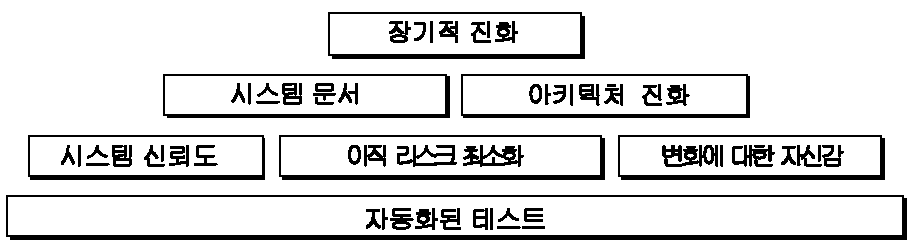
\includegraphics[width=\textwidth]{TestingFoundation}
\caption{Automated tests are the \emph{foundation} for reengineering. They establish your confidence in the system, reduce risks, and improve confidence in your ability to change the system. }
\figlabel{TestingFoundation}
\end{center}
\end{figure}

\noindent
Tests represent confidence in a system, because they specify how parts of the system work in a \emph{verifiable} way, and because they can be run at any time to check if the system is still consistent. 

\index{Davis, Alan}
\begin{quotation}
\noindent
\emph{``... testing simply exposes the presence of flaws in a program; it cannot be used to verify the absence of flaws. It can increase your confidence that a program is correct''}

\hfill --- Alan Davis, Principle 111 \cite{Davi95a}
\end{quotation}

Systematic testing is heavily promoted by \ind{Extreme Programming} \cite{Beck00a} one of the basic techniques necessary to be able to adapt programs quickly to changing requirements. Changing legacy systems is risky business. Will the code still work after a change? How many unexpected side-effects will appear? Having a set of automated, repeatable tests helps to reduce this risk. 

\begin{bulletlist}
\item A set of running tests provides confidence in the system. (``Are you really sure this piece of code works?'' ``Yes, look, here I have the tests that prove it.'')
\item A set of running tests represents \emph{reproducible} and \emph{verifiable} information about your system, and is at all times in sync with the application. This in contrast to most of the written documentation, which is typically slightly outdated already the next day.
\item Writing tests increases productivity, because bugs are found much earlier in the development process.
\end{bulletlist}

\subsection*{Related Patterns}

\patref{Write Tests to Enable Evolution}{WriteTestsToEnableEvolution} is a prerequisite to \patpgref{Always Have a Running Version}{AlwaysHaveARunningVersion}. Only with a comprehensive test program in place can you \patpgref{Migrate Systems Incrementally}{MigrateSystemsIncrementally}. 

\patref{Grow Your Test Base Incrementally}{GrowYourTestBaseIncrementally} and \patref{Test the Interface, Not the Implementation}{TestTheInterfaceNotTheImplementation} introduce a way to incrementally build a test suite while a system is evolving. 

%=================================================================
%:PATTERN -- {Grow Your Test Base Incrementally}
\pattern{Grow Your Test Base Incrementally}{GrowYourTestBaseIncrementally}


\intent{Balance the costs and the benefits of tests by incrementally introducing just the tests you need at a given point in time.}

\subsection*{Problem}

When should you start to introduce tests? When can you stop?

\emph{This problem is difficult because:}

\begin{bulletlist}
\item In a reengineering project, you cannot afford to spend too much time for writing tests.
\item Legacy systems tend to be huge, so testing everything is impossible.
\item Legacy systems tend to be poorly-documented and poorly-understood.
\item The original developers may have left and the system maintainers may have only limited knowledge of the system's inner workings.
\end{bulletlist}

\emph{Yet, solving this problem is feasible because:}

\begin{bulletlist}
\item We know where the fragile parts or the parts that we would like to change are.
\item We could convince programmers that they can benefit from tests.
\end{bulletlist}

\subsection*{Solution}

Introduce tests incrementally for parts of the system you are working on.

\subsubsection*{Hints}

\begin{bulletlist}
\item Carefully assess your priorities and initially develop tests only for the most critical components. As you reengineer the system, introduce tests for the new features, parts of the legacy that may be affected, and any bugs you identify along the way. 
\item Keep a snapshot of the old system handy so you can later introduce tests that should run against both the original system and its new incarnation.
\item Focus on business values. Start to write tests for the parts of your system that have the most important artifacts. Try to \patref{Record Business Rules as Tests}{RecordBusinessRulesAsTests}.
\item If you have the history of bug fixes or problems, apply \patpgref{Test Old Bugs}{TestOldBugs} as a starting point.
\item If you have acceptable documentation and some original developers of the system at hand, consider applying \patpgref{Test Fuzzy Features}{TestFuzzyFeatures}.
\item Apply \patref{Test the Interface, Not the Implementation}{TestTheInterfaceNotTheImplementation}, start to test big abstractions and then refine tests if time allows. For example, if you have a pipeline architecture, start to write tests that ensure you that the output of the full pipeline is right given the right input. Then write tests for the individual pipeline components.
\item Black-box test parts (subsystems, classes, methods) that are likely to change their implementation in the future.
\index{black box testing}
\end{bulletlist}

\subsection*{Tradeoffs}

\subsubsection*{Pros}

\begin{bulletlist}
\item You save time by only developing the tests that you need.
\item You build up a base of the most critical tests as the project progresses.
\item You build confidence as you go along
\item You streamline future development and maintenance activities.
\end{bulletlist}

\subsubsection*{Cons}

\begin{bulletlist}
\item You may guess wrong which aspects are critical to test.
\item Tests can give you false confidence --- untested bugs can still lurk in the system.
\end{bulletlist}

\subsubsection*{Difficulties}

\begin{bulletlist}
\item Setting-up the proper context for the tests may require considerable time and effort.
\item Identifying the boundaries of the components to test is just hard. Deciding which parts to test and how fine-grained these tests should be, requires a good understanding of the system and the way you intend to reengineer it.
\end{bulletlist}

\subsection*{Example}

\begin{figure}[h]
\begin{center}
\includegraphics[width=0.8\textwidth]{TestingChange}
\caption{Introduce tests for the parts of the system you intend to change.}
\figlabel{TestingChange}
\end{center}
\end{figure}

Initially introduce tests only for the subsystems and component you intend to change. In \figref{TestingChange} we introduce some tests for subsystem ABC and for its component B. We apply \patref{Test the Interface, Not the Implementation}{TestTheInterfaceNotTheImplementation} to ensure that the tests for B should also pass for newB.

Note that if we only introduce tests for component B, then we fail to test its integration with A and C. In any case, it may be that we fail to test all important aspects, so it is important to incrementally add new tests as bugs are detected and repaired.

\subsection*{Rationale}

An incremental testing strategy allows you to start reengineering efforts before all the tests are in place. By focussing on just those tests that concern the parts of the system you are currently changing, you enable change with a minimal investment in testing, while help your team build confidence as you grow your tests base.

\subsection*{Related Patterns}

\patref{Use a Testing Framework}{UseATestingFramework} to organize your tests. 

\patref{Test the Interface, Not the Implementation}{TestTheInterfaceNotTheImplementation} provides a strategy for developing tests at arbitrary granularities. \patref{Record Business Rules as Tests}{RecordBusinessRulesAsTests} provides another strategy for testing components that implement business logic. \patref{Write Tests to Understand}{WriteTestsToUnderstand} helps you prime a test base while you are still reverse engineering the system.

%=================================================================
%:PATTERN -- {Use a Testing Framework}
\pattern{Use a Testing Framework}{UseATestingFramework}

\intent{Encourage developers to write and use regression tests by providing a framework that makes it easy to develop, organize and run tests.}

\subsection*{Problem}

How do you encourage your team to adopt systematic testing?

\emph{This problem is difficult because:} 

\begin{bulletlist}
\item Tests are boring to write.
\item Tests may require a considerable test data to be built up and torn down.
\item It may be hard to distinguish between test failures and unexpected errors.
\end{bulletlist}

\emph{Yet, solving this problem is feasible because:}

\begin{bulletlist}
\item Most tests follow the same basic pattern: create some test data, perform some actions, see if the results match your expectations, clean up the test data.
\item Very little infrastructure is needed to run tests and report failures and errors.
\end{bulletlist}

\subsection*{Solution}

Use a testing framework that allows suites of tests to be composed from individual test cases.

\subsubsection*{Steps}

Unit testing frameworks, like \ind{JUnit} and \ind{SUnit} \cite{Beck98a}, and various commercial test harness packages are available for most programming languages. If a suitable testing framework is not available for the programming language you are using, you can easily brew your own according to the following principles:

\begin{bulletlist}
\item The user must provide test cases that set up test data, exercise them, and make assertions about the results
\item The testing framework should wrap test cases as tests which can distinguish between assertion failures and unexpected errors.
\item The framework should provide only minimal feedback if tests succeed.

\begin{bulletlist}
\item Assertion failures should indicate precisely which test failed.

\item Errors should result in more detailed feedback (such as a full stack trace).
\end{bulletlist}

\item The framework should allow tests to be composed as test suites.
\end{bulletlist}

\subsection*{Tradeoffs}

\subsubsection*{Pros}

\begin{bulletlist}
\item A testing framework simplifies the formulation of tests and encourages programmers to write tests and use them.
\end{bulletlist}

\subsubsection*{Cons}

\begin{bulletlist}
\item Testing requires commitment, discipline and support. You must convince your team of the need and benefits of disciplined testing, and you must integrate testing into your daily process. One way of supporting this discipline is to have one testing coach in your team; consider this when you \patpgref{Appoint a Navigator}{AppointANavigator}.
\end{bulletlist}

\subsection*{Example}

\begin{figure}[tb]
\begin{center}
\includegraphics[width=\textwidth]{TestingJUnit}
\caption{JUnit is a popular testing framework for Java that offers much more flexibility than the minimal scheme described above.}
\figlabel{TestingJUnit}
\end{center}
\end{figure}

\ind{JUnit} is a popular testing framework for Java, which considerable enhances the basic scheme described above. \figref{TestingJUnit} shows that the framework requires users to define their tests as subclasses of \lct{TestCase}. Users must provide the methods \lct{setUp()}, \lct{runTest()} and \lct{tearDown()}. The default implementation of \lct{setup()} and \lct{tearDown()} are empty, and the default implementation of \lct{runTest()} looks for and runs a method which is the name of the test (given in the constructor). These user-supplied hook methods are then called by the \lct{runBare()} template method.

JUnit manages the reporting of failures and errors with the help of an additional \lct{TestResult} class. In the design of JUnit, it is an instance of \lct{TestResult} that actually runs the tests and logs errors or failures. In \figref{TestingTestrun} we see a scenario in which a \lct{TestCase}, in its run method, passes control to an instance of \lct{TestResult}, which in turn calls the \lct{runBare} template method of the \lct{TestCase}.

\begin{figure}[tb]
\begin{center}
\includegraphics[width=\textwidth]{TestingTestrun}
\caption{In JUnit, tests are actually run by an instance of \lct{TestResult}, which invokes the \lct{runBare} template method of a \lct{TestCase}. The user only needs to provide the \lct{setUp()} and \lct{tearDown()} methods, and the test method to be invoked by \lct{runTest()}.}
\figlabel{TestingTestrun}
\end{center}
\end{figure}

\lct{TestCase} additionally provides a set of different kinds of standard assertion methods, such as \lct{assertEquals}, \lct{assertFails}, and so on. Each of these methods throws an \lct{AssertionFailedError}, which can be distinguished from any other kind of exception.

In order to use the framework, we will typically define a new class, say \lct{TestHashtable}, that bundles a set of test suites for a given class, \lct{Hashtable}, that we would like to test. The test class should extend \lct{junit.framework.TestCase}:

\begin{code}
import junit.framework.*;
import java.util.Hashtable;

public class TestHashtable extends TestCase {
\end{code}

The instance variables of the test class will hold the fixture - the actual test data:

\begin{code}
	private Hashtable boss;
	private String joe = "Joe";
	private String mary = "Mary";
	private String dave = "Dave";
	private String boris = "Boris";
\end{code}

There should be constructor that takes the name of a test case as its parameter. Its behavior is defined by its superclass:

\begin{code}
	public TestHashtable(String name) {
		super(name);
	}
\end{code}

The \lct{setUp()} \ind{hook method} can be overridden to set up the fixture. If there is any cleanup activity to be performed, we should also override \lct{tearDown()}. Their default implementations are empty.

\begin{code}
	protected void setUp() {
		boss = new Hashtable();
	}
\end{code}

We can then define any number of test cases that make use of the fixture. Note that each test case is independent, and will have a fresh copy of the fixture. (In principle, we should design tests that not only exercise the entire interface, but the test data should cover both typical and boundary cases. The sample tests shown here are far from complete.) 

Each test case should start with the characters ``test":

\begin{code}
	public void testEmpty() {
		assert(boss.isEmpty());
		assertEquals(boss.size(), 0);
		assert(!boss.contains(joe));
		assert(!boss.containsKey(joe));
	}

	public void testBasics() {
		boss.put(joe, mary);
		boss.put(mary, dave);
		boss.put(boris, dave);
		assert(!boss.isEmpty());
		assertEquals(boss.size(), 3);
		assert(boss.contains(mary));
		assert(!boss.contains(joe));
		assert(boss.containsKey(mary));
		assert(!boss.containsKey(dave));
		assertEquals(boss.get(joe), mary);
		assertEquals(boss.get(mary), dave);
		assertEquals(boss.get(dave), null);
	}
\end{code}

You may provide a static method \lct{suite()} which will build an instance of \lct{junit.framework.TestSuite} from the test cases defined by this class:

\begin{code}
	public static TestSuite suite() {
		TestSuite suite = new TestSuite();
		suite.addTest(new TestHashtable("testBasics"));
		suite.addTest(new TestHashtable("testEmpty"));
		return suite;
	}
}
\end{code}

The test case class should be compiled, together with any class it depends on.

\begin{figure}
\begin{center}
\includegraphics[width=0.8\textwidth]{TestingTestRunner}
\caption{An instance of \lct{java.ui.TestRunner}.}
\figlabel{TestingTestRunner}
\end{center}
\end{figure}

To run the tests, we can start up any one of a number of \emph{test runner} classes provided by the JUnit framework, for instance \lct{junit.ui.TestRunner} (see \figref{TestingTestRunner}).

\begin{figure}
\begin{center}
\includegraphics[width=0.8\textwidth]{TestingSuccess}
\caption{A successful test run.}
\figlabel{TestingSuccess}
\end{center}
\end{figure}

This particular test runner expects you to type in the name of the test class. You may then \emph{run} the tests defined by this class. The test runner will look for the suite method and use it to build an instance of \lct{TestSuite}. If you do not provide a static \lct{suite} method, the test runner will automatically build a test suite assuming that all the methods named test* are test cases. The test runner then runs the resulting test suite. The interface will report how many tests succeeded (see \figref{TestingSuccess}). A successful test run will show a green display. If any individual test fails, the display will be red, and details of the test case leading to the failure will be given.

\subsection*{Rationale}

A testing framework makes it easier to organize and run tests. 

Hierarchically organizing tests makes it easier to run just the tests that concern the part of the system you are working on.

\subsection*{Known Uses}

Testing frameworks exist for a vast number of languages, including Ada, ANT, C, C++, Delphi, .Net (all languages), Eiffel, Forte 4GL, GemStone/S, Jade, JUnit Java, JavaScript, k language (ksql, from kbd), Objective C, Open Road (CA), Oracle, PalmUnit, Perl, PhpUnit, PowerBuilder, Python, Rebol, `Ruby, Smalltalk, Visual Objects and UVisual Basic.

Beck and Gamma give a good overview in the context of JUnit \cite{Beck98a}.

%=================================================================
%:PATTERN -- {Test the Interface, Not the Implementation}
\pattern{Test the Interface, Not the Implementation}{TestTheInterfaceNotTheImplementation}

\emph{Also Known As:}  Black-Box Testing \cite{Pres94a}

\intent{Build up reusable tests that focus on external behavior rather than on implementation details, and thereby will survive changes to the system.}

\subsection*{Problem}

How can you develop tests that not only protect your software legacy, but also will continue to be valuable as the system changes?

\emph{This problem is difficult because:}

\begin{bulletlist}
\item Legacy systems have many features that should continue to function as the system evolves.
\item You cannot afford to spend too much time writing tests while reengineering the system.
\item You do not want to waste effort in developing tests that will have to be changed as you change the system.
\end{bulletlist}

\emph{Yet, solving this problem is feasible because:}

\begin{bulletlist}
\item The interfaces to the components of the system tell you what should be tested.
\item Interfaces tend to be more stable than implementations
\end{bulletlist}

\subsection*{Solution}

Develop black-box tests that exercise the public interface of your components.

\subsubsection*{Hints}

\begin{bulletlist}
\item Be sure to exercise boundary values (\ie minimum and maximum values for method parameters). The most common errors occur here.
\item Use a top-down strategy to develop black-box tests if there are many fine-grained components that you do not initially have time to develop tests for.
\item Use a bottom-up strategy if you are replacing functionality in a very focussed part of the legacy system.
\end{bulletlist}

\subsection*{Tradeoffs}

\subsubsection*{Pros}

\begin{bulletlist}
\item Tests that exercise public interfaces are more likely to be reusable if the implementation changes.
\item Black-box tests can often be used to exercise multiple implementations of the same interface.
\item It is relatively easy to develop tests based on a component's interface.
\item Focusing on the external behavior reduces considerably the possible tests to be written while still covering the essential aspects of a system.
\end{bulletlist}

\subsubsection*{Cons}

\begin{bulletlist}
\item Back-box tests will not necessarily exercise all possible program paths. You may have to use a separate coverage tool to check whether your tests cover all the code.
\item If the interface to a component changes you will still have to adapt the tests.
\end{bulletlist}

\subsubsection*{Difficulties}

\begin{bulletlist}
\item Sometimes the class does not provide the right interface to support black-box testing. Adding accessors to sample the state of the object can be a simple solution, but this generally weakens encapsulation and makes the object less of a black box.
\end{bulletlist}

\subsection*{Example}

Let's look back at the test presented in \patref{Write Tests to Enable Evolution}{WriteTestsToEnableEvolution}. The code we saw earlier was supposed to check whether the add operation defined on a class \lct{Money} works as expected. However, we see that the assert in line (3) actually depends on the internal implementation of the \lct{Money} class, because it checks for equality by accessing the parts of equality.

\begin{code}
public class MoneyTest extends TestCase {
	// ...
		public void testSimpleAdd() {
			Money m12CHF= new Money(12, "CHF");                 // (1)
			Money m14CHF= new Money(14, "CHF");        
			Money expected= new Money(26, "CHF");
			Money result= m12CHF.add(m14CHF);                      // (2)
			assert(result.currency().equals(expected.currency())
				&& result.amount() == expected.amount());            // (3)
		}
}
\end{code}

However, if the class \lct{Money} would override the default \lct{equals} operation defined on \lct{Object} (doing so would also require us to override \lct{hashCode}), the last assert statement could be simplified and would become independent of the internal implementation.

\begin{code}
public class MoneyTest extends TestCase {
	// ...
		public void testSimpleAdd() {
			Money m12CHF= new Money(12, "CHF");            // (1)
			Money m14CHF= new Money(14, "CHF");        
			Money expected= new Money(26, "CHF");
			Money result= m12CHF.add(m14CHF);                // (2)
			assert(expected.equals(result));                            // (3)
		}
}
\end{code}

\subsection*{Rationale}

The interface of a component is a direct consequence of its collaborations with other components. Black-box tests therefore have a good chance of exercising the most important interactions of a system.

Since interfaces tend to be more stable than implementations, black-box tests have a good chance of surviving major changes to the system, and they thereby protect your investment in developing tests.

\subsection*{Known Uses}

Black-Box testing is a standard testing strategy \cite{Somm96a}.

\subsection*{Related Patterns}

\patref{Record Business Rules as Tests}{RecordBusinessRulesAsTests} adopts a different strategy to developing tests which focuses on exercising business rules. This is fine if the components to be tested are the ones that implement the business logic. For most other components, \patref{Test the Interface, Not the Implementation}{TestTheInterfaceNotTheImplementation} will likely be more appropriate.

\index{black box testing}
\index{white box testing}
Components that implement complex algorithms may not be well-suited to black-box testing, since an analysis of the interface alone may not reveal all the cases that the algorithm should handle. White-box testing \cite{Somm96a} is another standard technique for testing algorithms in which test cases are generated to cover all possible paths through an algorithm.

%=================================================================
%:PATTERN -- {Record Business Rules as Tests}
\pattern{Record Business Rules as Tests}{RecordBusinessRulesAsTests}


\intent{Keep the system in sync with the business rules it implements by encoding the rules explicitly as tests.}

\subsection*{Problem}

How do you keep the \emph{actual business rules}, the \emph{documentation} about those business rules and the system \emph{implementation} in sync, while all three are changing?

\emph{This problem is difficult because:}

\begin{bulletlist}
\item Written documentation gets out of date quickly and does not ensure you that your system really implements the description of the business rules you have.
\item Business rules tend to be implicit in the code. It may not be obvious which pieces of software are responsible for computing a given business rule.
\item Developer turn-over introduces a high risk for your business by having more and more people knowing less and less about the system.
\item Most of the time only one programmer or user knows specific rules, and that person could be leaving tomorrow.
\item Business rules are likely to change due to external factors, such as the introduction of a new law, so it is important to represent them explicitly.
\end{bulletlist}

\emph{Yet, solving this problem is feasible because:}

\begin{bulletlist}
\item Most business rules are well expressed by sets of canonical examples, each of which requires certain well-defined actions to be taken, and results in some clear, observable results.
\end{bulletlist}

\subsection*{Solution}

Write executable tests that record the business rules as test cases, actions, and tests over the results. When tests break, you know that things are out of sync.

\subsubsection*{Hints}

\begin{bulletlist}
\item Developers and clients can write tests. Developers may write tests associated with specific functionality or piece of code. User may also have to write integration tests in the form of use cases that bind together several unit tests \cite{Davi95a} \cite{Beck00a}. 
\item Note that you are not interested in the implementation strategies or optimization aspects, but only the business rules. 
\end{bulletlist}

\subsection*{Tradeoffs}

\subsubsection*{Pros}

\begin{bulletlist}
\item The rules become explicit, thereby reducing dependency on human memory.
\item You need to record the business rules anyway before you can reengineer the legacy system.
\item Recording business rules as tests enables evolution: when new features must be added, you can check that the existing business rules are still correctly implemented by running the regression tests. On the other hand, when the business rules change, you can update the corresponding tests to reflect the changes.
\end{bulletlist}

\subsubsection*{Cons}

\begin{bulletlist}
\item Tests can only encode concrete scenarios, not actual the logic of the business rules themselves.
\item When the business logic must deal with an extremely large number of cases, it may be impractical to test them all.
\end{bulletlist}

\subsubsection*{Difficulties}

\begin{bulletlist}
\item Recording business rules does not mean extracting them. Extracting business rules from code with the current technology is a pipe dream.
\item Recording business rules can be difficult for system whose original developers and users have all left. 
\end{bulletlist}

\subsection*{Examples}

In this example we compute the amount of additional money an employee receives for a child. The rule states that a person or couple gets an amount of money for every child he, she or they raise. Basically parents get CHF 150,- per month for every child younger than 12 years, and CHF 180,- for every child between 12 and 18 and for every child between 18 and 25 as long as the child is not working and is still in the educational system. A single parent gets the full 100\% of this money as long as he or she is working more than 50\%. Couples get a percentage of the money that is equal to the summed working percentages of both partners.

The following \ind{Smalltalk} code shows a test that hardcodes the expected outcomes for the different computations. It allows for automatically checking the outcomes instead of having to print the outcomes and check by hand if they are right, and it acts as a regression test. Secondly it documents the expected outcome of the different computations.

\begin{code}
testMoneyGivenForKids
	|	singlePerson80occupationWithOneKidOf5
		couplePerson40occupationWithOneKidOf5
		couplePerson100occupationWith2KsidOf5
		couplePersonWithOneKidOf14 |

"cases are extracted from a database after the system has
performed the computation"

singlePerson80WithOneKidOf5 := extract....
couplePerson40occupationWithOneKidOf5 := extract....
couplePerson100occupationWithOneKidOf5 := extract....
couplePersonWithOneKidOf14 := extract....
"tests"

"We test that the right amount of money is computed correctly"

self assert: singlePerson80occupationWithOneKidOf5 moneyForKid = 150.
self assert: couplePerson40occupationWithOneKidOf5 moneyForKid = 150*4.
self assert: couplePerson100occupationWith2KidsOf5 moneyForKid = 150*2.
self assert: couplePersonWithOneKidOf14 moneyForKid = 180.
\end{code}

\subsection*{Rationale}

Tests are a good way to document what the system does. By documenting business rules as tests, you guarantee that the description of the business rules will be in sync with the implementation. 

The beginning of a reengineering project is a good point in time to set up a process to document knowledge about the system as explicit tests.

\subsection*{Related Patterns}

While you are reverse engineering a legacy system, you may \patref{Write Tests to Understand}{WriteTestsToUnderstand}. During this process it will be natural to \patref{Record Business Rules as Tests}{RecordBusinessRulesAsTests}. In this way you can prime your test base as you \patref{Grow Your Test Base Incrementally}{GrowYourTestBaseIncrementally}.

%=================================================================
%:PATTERN -- {Write Tests to Understand}
\pattern{Write Tests to Understand}{WriteTestsToUnderstand}

\intent{Record your understanding of a piece of code in the form of executable tests, thus setting the stage for future changes.}

\subsection*{Problem}

How do you develop an understanding of a part of a legacy system which contains neither tests nor accurate and precise documentation?

\emph{This problem is difficult because:}

\begin{bulletlist}
\item Code is always difficult to understand.
\item You would like to make hypotheses about what the code is really doing and validate them.
\item You would like to specify as precisely as possible the behavior of the system.
\item You would like to record your understanding to communicate it but you do not want to waste your time in writing documents that will be obsolete as soon as you start changing the code. 
\end{bulletlist}

\emph{Yet, solving this problem is feasible because:}

\begin{bulletlist}
\item The piece of code is relatively small and has clearly defined boundaries.
\item You have the possibility to specify tests and validate them.
\end{bulletlist}

\subsection*{Solution}

Encode your hypotheses and conclusions as executable tests.

\subsection*{Tradeoffs}

\subsubsection*{Pros}

\begin{bulletlist}
\item Tests help you to validate your understanding.
\item Tests can provide a precise specification of certain aspects of the system. Tests cannot be fuzzy.
\item Tests can be applied to gain different levels of understanding. For example, black-box tests can help you to refine your understanding of roles and collaborations, whereas white-box tests can help you to gain understanding of the implementation of complex logic.
\item The tests that you develop will help to enable future reengineering effort.
\item Tests will force you to be precise about the creation and the use of the objects under test.
\end{bulletlist}

\subsubsection*{Cons}

\begin{bulletlist}
\item Writing tests is time consuming.
\end{bulletlist}

\subsubsection*{Difficulties}

\begin{bulletlist}
\item Obtaining a well defined context in which you can test the objects is difficult especially if the objects to be tested do not represent specific abstractions. Looking for the places where objects you want to understand are created can help. 
\item Concurrent systems are known to be difficult to test, so tests can miss important aspects (such as handling of race conditions).
\end{bulletlist}

\subsection*{Rationale}

By writing automated tests, you exercise parts of the system you want to understand, while recording your understanding and setting the stage for future reengineering effort.

\subsection*{Related Patterns}

Before writing any tests, you might want to \patpgref{Refactor to Understand}{RefactorToUnderstand}. As you write your tests, be sure to \patpgref{Tie Code and Questions}{TieCodeAndQuestions}.

%=============================================================
\ifx\wholebook\relax\else
   \bibliographystyle{alpha}
   \bibliography{scg}
   \end{document}
\fi
%=============================================================
